\documentclass[11pt,a4paper]{article}
\usepackage[margin=2.5cm]{geometry}
\usepackage{graphicx}
\usepackage{booktabs}
\usepackage{longtable}
\usepackage{hyperref}
\usepackage{xcolor}
\usepackage{caption}
\usepackage{array}
\usepackage{tabularx}
\usepackage{float}

\hypersetup{
    colorlinks=true,
    linkcolor=blue,
    urlcolor=blue,
    citecolor=blue
}

\newcolumntype{L}[1]{>{\raggedright\arraybackslash}p{#1}}
\newcolumntype{C}[1]{>{\centering\arraybackslash}p{#1}}

\title{\textbf{Supplementary Information}\\[0.5em]
\large Audio Spectrogram Transformers for Voice-Based Disease Detection\\
Using Task-Specific Biomarkers Across Neurological and Psychiatric Conditions}
\author{Shikhar Shukla, Parvati Naliyatthaliyazchayil, Judy Gichoya, Saptarshi Purkayastha}
\date{}

\begin{document}
\maketitle

\tableofcontents
\newpage

%% ============================================================
%% SECTION 1: TRIPOD+AI CHECKLIST
%% ============================================================
\section{TRIPOD+AI Checklist}

This study is reported in accordance with the TRIPOD+AI guidelines for prediction model studies (Collins GS, et al. TRIPOD+AI statement: updated guidance for reporting clinical prediction models that use regression or machine learning methods. \textit{BMJ}. 2024;385:e078378).

\vspace{0.5em}
\noindent\textbf{Study type:} Development with internal validation (5-fold cross-validation).

\vspace{1em}

{
\small
\begin{longtable}{C{0.6cm} L{2.2cm} C{0.6cm} L{5.5cm} L{4.5cm}}
\toprule
\textbf{Item} & \textbf{Section} & \textbf{Type} & \textbf{Checklist Item} & \textbf{Reported (Page/Section)} \\
\midrule
\endfirsthead

\toprule
\textbf{Item} & \textbf{Section} & \textbf{Type} & \textbf{Checklist Item} & \textbf{Reported (Page/Section)} \\
\midrule
\endhead

\midrule
\multicolumn{5}{r}{\textit{Continued on next page}} \\
\endfoot

\bottomrule
\endlastfoot

%% TITLE
1 & Title & D;E & Identify the study as developing or evaluating the performance of a multivariable prediction model, the target population, and the outcome to be predicted & Title (p.~1). Title identifies AST-based disease detection model for neurological/psychiatric conditions. \\
\addlinespace

%% ABSTRACT
2 & Abstract & D;E & See TRIPOD+AI for Abstracts checklist & Abstract (p.~2). See Section~\ref{sec:abstract_checklist}. \\
\addlinespace

%% INTRODUCTION
3a & Introduction: Background & D;E & Explain the healthcare context and rationale for developing the prediction model, including references to existing models & Introduction (pp.~2--4). Diagnostic/screening context; speech as non-invasive biomarker; existing approaches referenced. \\
\addlinespace

3b & Introduction: Target population & D;E & Describe the target population and the intended purpose of the prediction model & Introduction (pp.~3--4). Target: individuals with PD, dementia, or depression; purpose: screening for further clinical evaluation. \\
\addlinespace

3c & Introduction: Health inequalities & D;E & Describe any known health inequalities between sociodemographic groups & Introduction. Speech biomarkers may vary with age, sex, language, and cultural background; noted as area for future investigation. \\
\addlinespace

4 & Introduction: Objectives & D;E & Specify the study objectives, including whether development or validation & Introduction (p.~4). Development with internal validation (5-fold CV) across three conditions. \\
\addlinespace

%% METHODS - DATA
5a & Methods: Data sources & D;E & Describe the sources of data, rationale, and representativeness & Methods: Dataset Description (p.~20). Bridge2AI Voice Dataset v2.0.0 (PhysioNet). Multi-site, publicly available. \\
\addlinespace

5b & Methods: Dates & D;E & Specify the dates of the collected participant data & Data collection dates described in the parent dataset publications [19,~20]. \\
\addlinespace

%% METHODS - PARTICIPANTS
6a & Methods: Study setting & D;E & Specify key elements of the study setting & Methods (p.~20). Multi-site dataset; specific site details in parent publications [19,~20]. \\
\addlinespace

6b & Methods: Eligibility & D;E & Describe the eligibility criteria for study participants & Methods: Task Selection (pp.~21--22). Spectrograms $\geq$100 time frames from selected high-prevalence tasks. \\
\addlinespace

6c & Methods: Treatments & D;E & Give details of any treatments received & Medication status not controlled. Noted as limitation (Discussion). \\
\addlinespace

%% METHODS - DATA PREP
7 & Methods: Data preparation & D;E & Describe any data pre-processing and quality checking & Methods: Preprocessing (pp.~22--24). Four-step pipeline: temporal standardization, frequency resizing, z-score normalization, final representation. Same for all participants. \\
\addlinespace

%% METHODS - OUTCOME
8a & Methods: Outcome definition & D;E & Clearly define the outcome being predicted and the time horizon & Methods (pp.~20--21). Binary classification from phenotype labels. Cross-sectional (no time horizon). \\
\addlinespace

8b & Methods: Outcome assessors & D;E & Describe qualifications of outcome assessors if subjective & N/A. Labels are self-reported condition status from phenotype file [19,~20]. \\
\addlinespace

8c & Methods: Blinding & D;E & Report any actions to blind assessment of the outcome & Methods: CV (p.~27). Strict participant-level separation; OOF predictions from models that never observed the participant. \\
\addlinespace

%% METHODS - PREDICTORS
9a & Methods: Predictor selection & D & Describe the choice of initial predictors & Methods (pp.~22--24). Full log-Mel spectrograms; no manual feature selection. LR baseline: 809 summary statistics. \\
\addlinespace

9b & Methods: Predictor definition & D;E & Clearly define all predictors & Methods (pp.~20, 22--24). Spectrograms: 128$\times$1024 Mel-frequency representations. \\
\addlinespace

9c & Methods: Predictor assessors & D;E & Describe qualifications of predictor assessors if subjective & N/A. Spectrograms are algorithmically derived; no subjective interpretation. \\
\addlinespace

%% METHODS - SAMPLE SIZE
10 & Methods: Sample size & D;E & Explain how the study size was arrived at & Methods (pp.~21--22); Discussion: Limitations. Determined by available dataset. No formal sample size calculation. Modest sizes acknowledged as limitation. \\
\addlinespace

%% METHODS - MISSING DATA
11 & Methods: Missing data & D;E & Describe how missing data were handled & Methods (p.~22). Spectrograms $<$100 frames excluded. Complete cases only. NaN in extracted features replaced with 0. \\
\addlinespace

%% METHODS - ANALYTICAL
12a & Methods: Data use & D & Describe how data were used and partitioned & Methods (pp.~24, 27). Preliminary 80/20 split for development only; all reported results from 5-fold CV on full cohort. \\
\addlinespace

12b & Methods: Predictor handling & D & Describe how predictors were handled & Methods (pp.~22--24). Z-score normalization per fold (training statistics only). StandardScaler for LR baseline. \\
\addlinespace

12c & Methods: Model type & D & Specify type of model, rationale, building steps, hyperparameter tuning, internal validation & Methods (pp.~24--27). AST (ViT backbone, AudioSet pretrained). AdamW, differential LR, focal loss, SpecAugment, early stopping. 5-fold CV. Fixed hyperparameters. \\
\addlinespace

12d & Methods: Heterogeneity & D;E & Describe how heterogeneity in model performance was handled across clusters & Results (pp.~5--9). Per-fold metrics with mean, SD, 95\% CI. Fold-level variability discussed. No multi-centre analysis. \\
\addlinespace

12e & Methods: Performance measures & D;E & Specify all measures and plots used & Methods (p.~27); Results (pp.~5--12). AUC-ROC, F1, precision, recall, Brier scores, calibration curves, ROC/PR curves, confusion matrices. \\
\addlinespace

12f & Methods: Model updating & E & Describe any model updating & N/A. Development study; no updating performed. \\
\addlinespace

12g & Methods: Predictions & E & Describe how predictions were calculated & N/A (development). Full code publicly available on GitHub. \\
\addlinespace

%% METHODS - CLASS IMBALANCE
13 & Methods: Class imbalance & D;E & State why and how class imbalance was addressed & Methods: Training (p.~26). Weighted random sampler, focal loss with dynamic class weights ($w_c = N_{\text{total}} / (2 \times n_c)$), class\_weight=`balanced' for LR. No post-hoc recalibration. \\
\addlinespace

%% METHODS - FAIRNESS
14 & Methods: Fairness & D;E & Describe approaches used to address model fairness & Partially addressed. Demographic metadata analysis showed near-chance AUC (0.592), suggesting model does not proxy for age/sex. No formal fairness assessment. \\
\addlinespace

%% METHODS - MODEL OUTPUT
15 & Methods: Model output & D & Specify output of the prediction model and threshold identification & Methods (p.~27). Participant-level probability (mean of recording-level softmax). Thresholds via Youden's J on OOF predictions. \\
\addlinespace

%% METHODS - DEV VS EVAL
16 & Methods: Dev vs.\ eval & D;E & Identify differences between development and evaluation data & Methods (p.~27). Same dataset via 5-fold CV. No external validation. Fold-specific normalization. \\
\addlinespace

%% METHODS - ETHICS
17 & Methods: Ethics & D;E & Name ethics committee that approved the study & Data Availability (p.~29). USF IRB approved parent study. De-identified public data; no additional IRB required. \\
\addlinespace

%% OPEN SCIENCE
18a & Open Science: Funding & D;E & Give source of funding and role of funders & Acknowledgments (p.~29). NIH, RWJF, RSNA, Lacuna Fund, Moore Foundation grants listed. \\
\addlinespace

18b & Open Science: Conflicts & D;E & Declare conflicts of interest & Competing Interests (p.~30). P.N. employed at ConcertAI (independent); others declare none. \\
\addlinespace

18c & Open Science: Protocol & D;E & Indicate where protocol can be accessed & No formal study protocol was prepared prior to the analysis. \\
\addlinespace

18d & Open Science: Registration & D;E & Provide registration information & This study was not pre-registered in a prediction model registry. \\
\addlinespace

18e & Open Science: Data & D;E & Provide details of data availability & Data Availability (p.~29). PhysioNet, DOI: 10.13026/3xt6-rf05. \\
\addlinespace

18f & Open Science: Code & D;E & Provide details of code availability & Code Availability (p.~29). GitHub: Amorfati123/bridge2ai-voice-parkinsons-ast. \\
\addlinespace

%% PPI
19 & Patient/Public Involvement & D;E & Provide details of PPI or state no involvement & No patient or public involvement in the design, conduct, reporting, or dissemination of this research. \\
\addlinespace

%% RESULTS - PARTICIPANTS
20a & Results: Participant flow & D;E & Describe flow of participants & Results: Cohort Characteristics (pp.~4--5). 442 total; condition-specific cohorts described with exclusion criteria. \\
\addlinespace

20b & Results: Characteristics & D;E & Report characteristics overall and for each setting & Results: Tables 3, 6 (pp.~4--5, 9--10). Case/control distributions, recording counts. \\
\addlinespace

%% RESULTS - MODEL DEV
21 & Results: Sample sizes & D;E & Specify number of participants and events in each analysis & Results (pp.~5--10). Per-fold train/val splits reported. Sensitivity analysis: 442 participants. Baselines: 112 participants. \\
\addlinespace

%% RESULTS - MODEL SPEC
22 & Results: Model specification & D & Provide details of full prediction model & Code Availability (p.~29); Methods (pp.~24--27). Architecture, checkpoint, and code all publicly available. \\
\addlinespace

%% RESULTS - PERFORMANCE
23a & Results: Performance & D;E & Report performance estimates with confidence intervals & Results: Tables 4, 5 (pp.~7--8). Per-fold and OOF metrics with SD and 95\% CI. Baseline comparison table. Calibration (Brier scores). \\
\addlinespace

23b & Results: Heterogeneity & D;E & Report heterogeneity in model performance & Results: Table 4; Figure 4. Per-fold variability reported. Depression: extreme heterogeneity (AUC 0.321--0.963). \\
\addlinespace

%% RESULTS - UPDATING
24 & Results: Updating & E & Report results from any model updating & N/A. Development study; no updating performed. \\
\addlinespace

%% DISCUSSION
25 & Discussion: Interpretation & D;E & Give overall interpretation including fairness & Discussion (pp.~13--19). Comprehensive interpretation with prior work comparison and baseline gap analysis. \\
\addlinespace

26 & Discussion: Limitations & D;E & Discuss limitations and effects on biases, uncertainty, and generalisability & Discussion (pp.~17--18). Nine limitations discussed including cohort size, single dataset, task selection circularity, comorbidity, medication, language. \\
\addlinespace

27a & Discussion: Input quality & D & Describe handling of poor quality or unavailable input data & Methods (p.~22). Minimum 100-frame threshold. Discussion notes that behavior on degraded recordings is uncharacterized. \\
\addlinespace

27b & Discussion: User interaction & D & Specify user interaction requirements and expertise level & Discussion. Automated pipeline; clinical interpretation of outputs requires clinical expertise. \\
\addlinespace

27c & Discussion: Next steps & D;E & Discuss next steps for future research & Discussion (pp.~18--19). Task design, external validation, interpretability, longitudinal monitoring, Bridge2AI v3.0.0 replication. \\

\end{longtable}
}

\subsection{TRIPOD+AI for Abstracts Checklist}
\label{sec:abstract_checklist}

{
\small
\begin{longtable}{L{3cm} L{5cm} C{1.5cm} L{4.5cm}}
\toprule
\textbf{Item} & \textbf{Requirement} & \textbf{Reported?} & \textbf{Location} \\
\midrule
\endfirsthead
\endhead

Study design & Identify whether the study developed or validated a prediction model & Yes & ``We applied a pretrained Audio Spectrogram Transformer'' \\
\addlinespace
Participants & Describe the study participants and setting & Yes & ``Bridge2AI Voice Dataset'' with condition-specific cohorts \\
\addlinespace
Outcome & State the outcome to be predicted & Yes & PD, dementia, depression screening \\
\addlinespace
Predictors & Describe the predictors & Yes & ``spectrogram-based'' AST framework \\
\addlinespace
Sample size & Report number of participants and outcome events & Partial & Cohort sizes implied from AUC reports; not explicitly stated \\
\addlinespace
Model type & Describe the type of prediction model & Yes & ``Audio Spectrogram Transformer (AST)'' \\
\addlinespace
Performance & Provide performance measures with confidence intervals & Partial & OOF AUC reported for all conditions and baselines; CIs not in abstract \\
\addlinespace
Conclusions & Provide an overall interpretation & Yes & Task selection as central design decision \\
\bottomrule
\end{longtable}
}


%% ============================================================
%% SECTION 2: SUPPLEMENTARY FIGURES
%% ============================================================
\newpage
\section{Supplementary Figures}

%% --- FIGURE S1: BASELINE ROC ---
\begin{figure}[H]
\centering
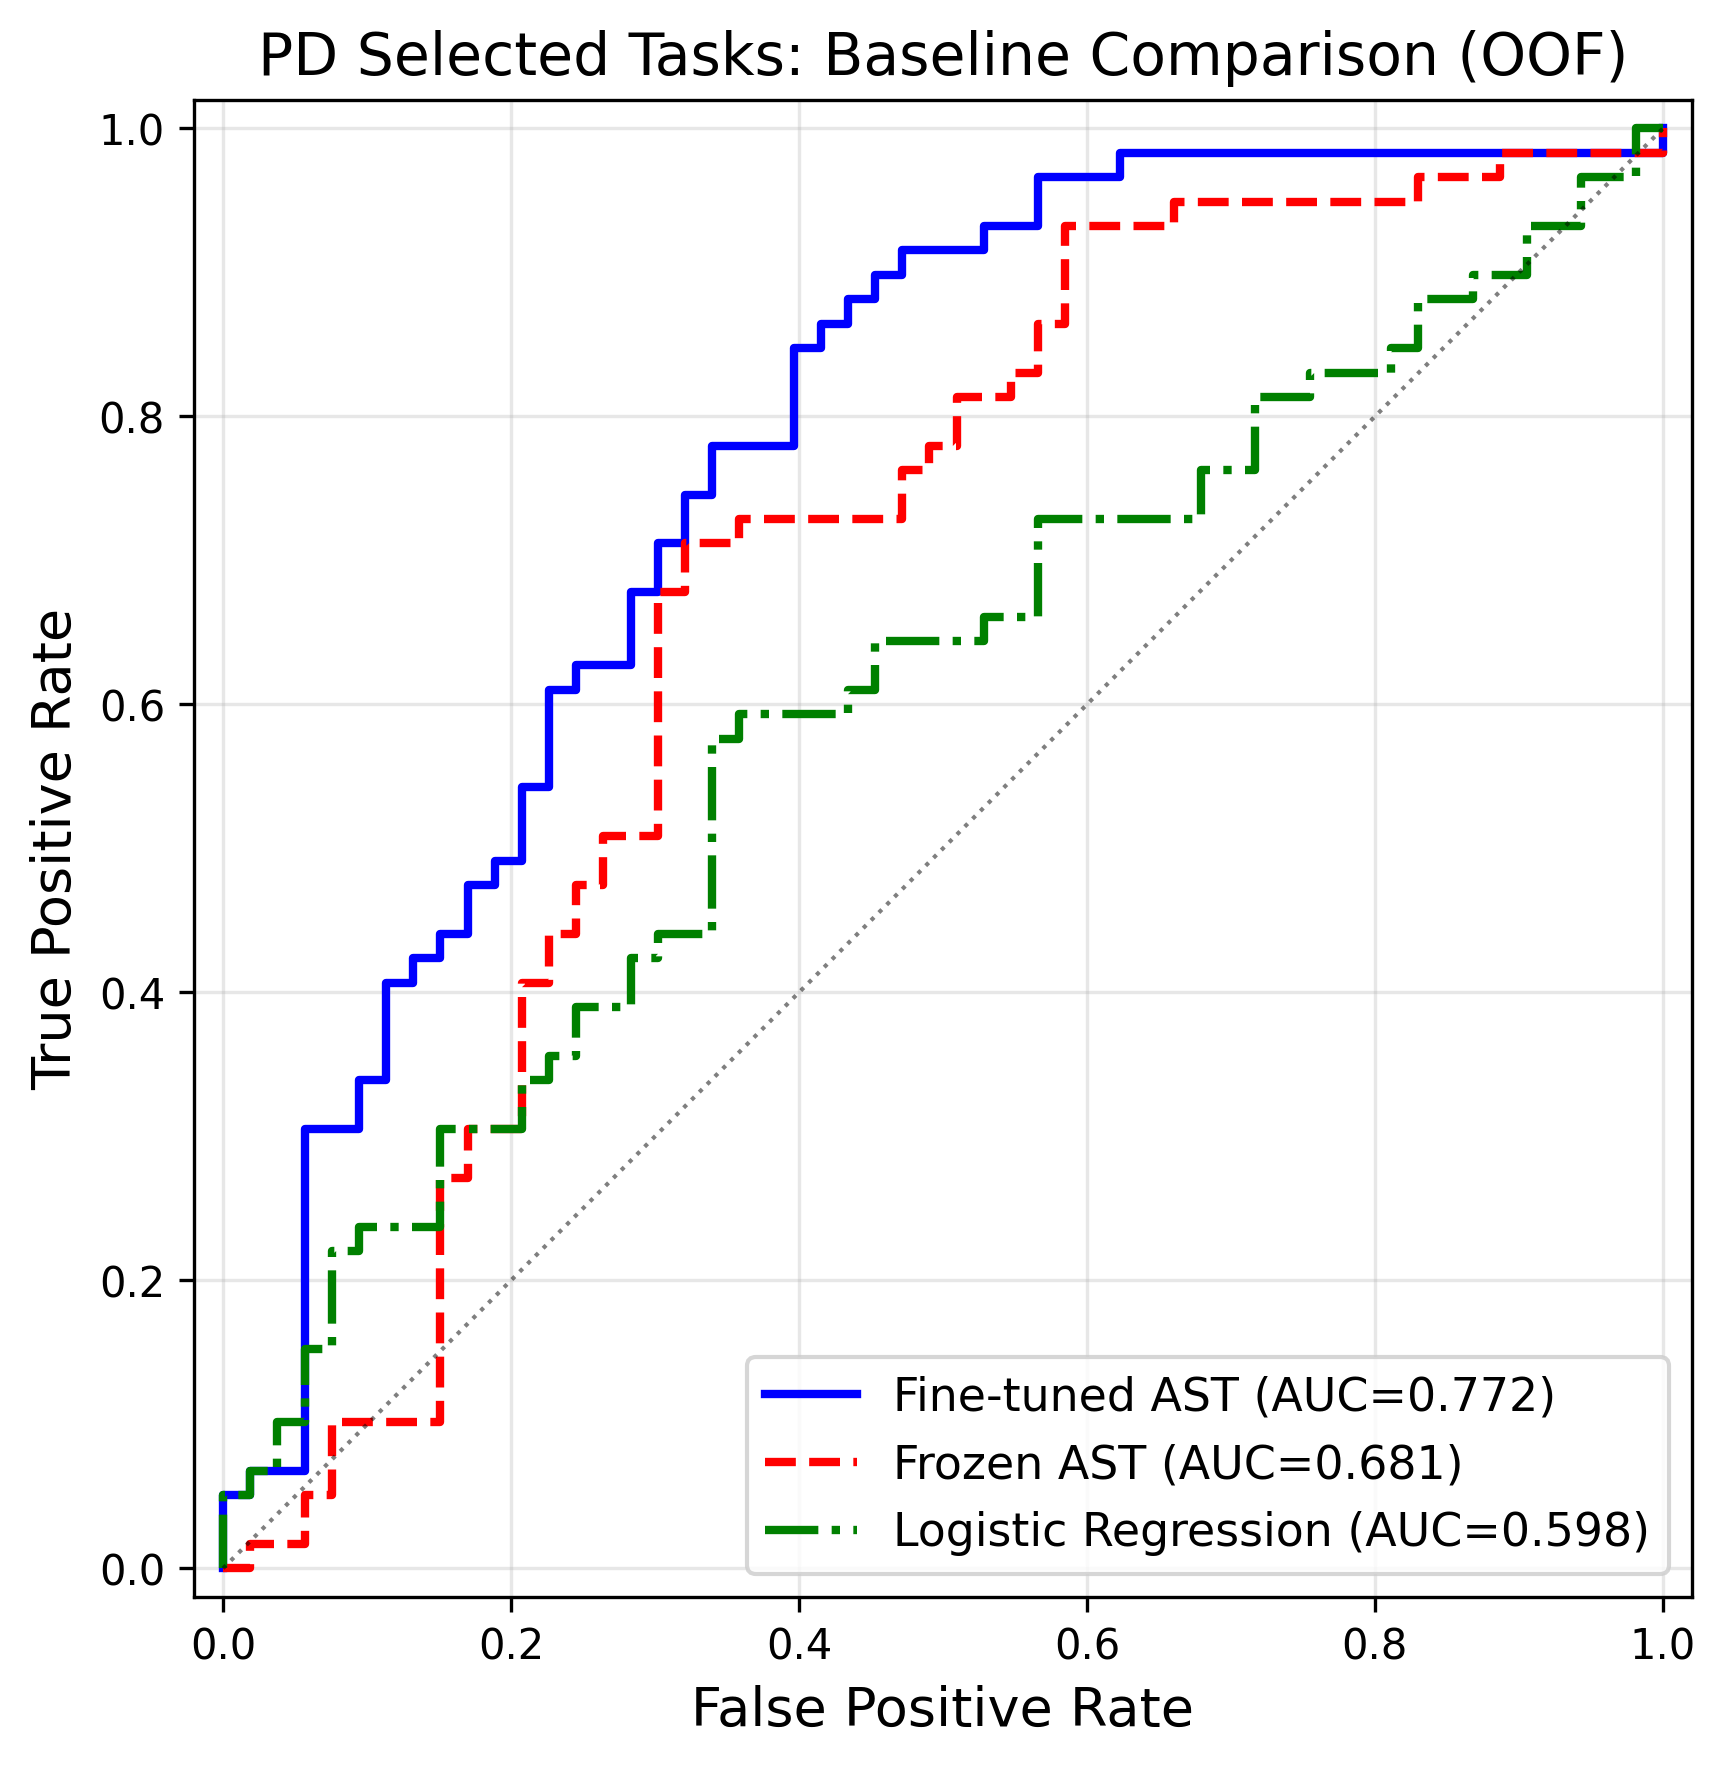
\includegraphics[width=0.65\textwidth]{baseline_roc_comparison.png}
\caption{\textbf{Supplementary Figure S1. Baseline comparison of ROC curves for PD screening (selected tasks).}
Participant-level out-of-fold receiver operating characteristic curves for three models evaluated using identical five-fold cross-validation splits (random\_state = 42): fine-tuned AST (AUC = 0.772), frozen AST with linear probing (AUC = 0.681), and logistic regression on spectrogram summary statistics (AUC = 0.598). The fine-tuning gap (+0.091 AUC) demonstrates the benefit of domain adaptation to clinical speech beyond pretrained AudioSet features. The deep learning gap (+0.174 AUC) confirms that learned representations capture discriminative patterns not available from handcrafted statistics.}
\label{fig:baseline_roc}
\end{figure}

\vspace{1em}

%% --- FIGURE S2: CALIBRATION ---
\begin{figure}[H]
\centering
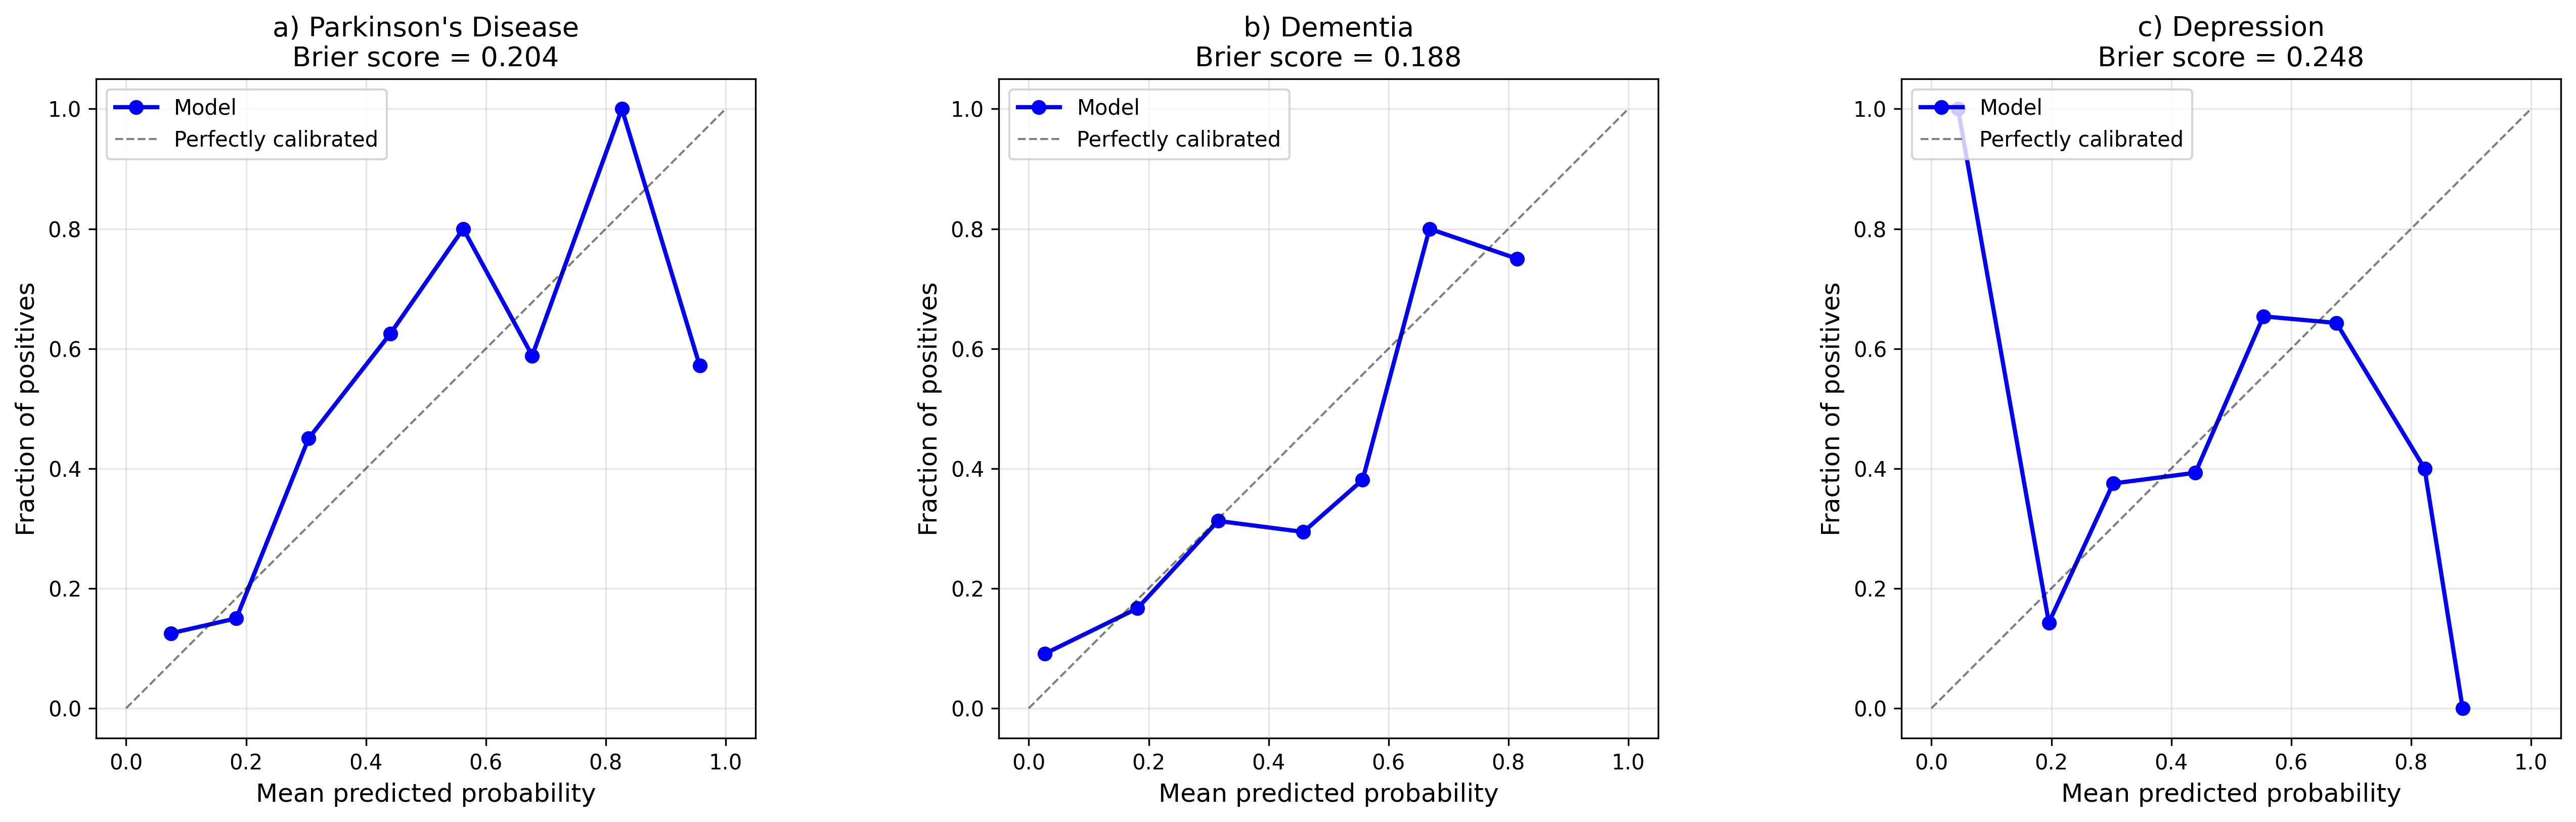
\includegraphics[width=\textwidth]{calibration_curves.png}
\caption{\textbf{Supplementary Figure S2. Calibration curves for all three conditions.}
Reliability diagrams and Brier scores computed from out-of-fold predictions of the fine-tuned AST.
(a) Parkinson's disease (Brier score = 0.204): reasonable calibration with slight overconfidence in the 0.6--0.8 probability range.
(b) Dementia (Brier score = 0.188): best-calibrated model, with predicted probabilities tracking observed event rates.
(c) Depression (Brier score = 0.248): least well-calibrated, consistent with the instability of the underlying predictions.
Ten equal-width bins were used. The dashed diagonal represents perfect calibration. Lower Brier scores indicate better calibration (range 0--1).}
\label{fig:calibration}
\end{figure}

\newpage

%% --- FIGURE S3: PER-TASK ---
\begin{figure}[H]
\centering
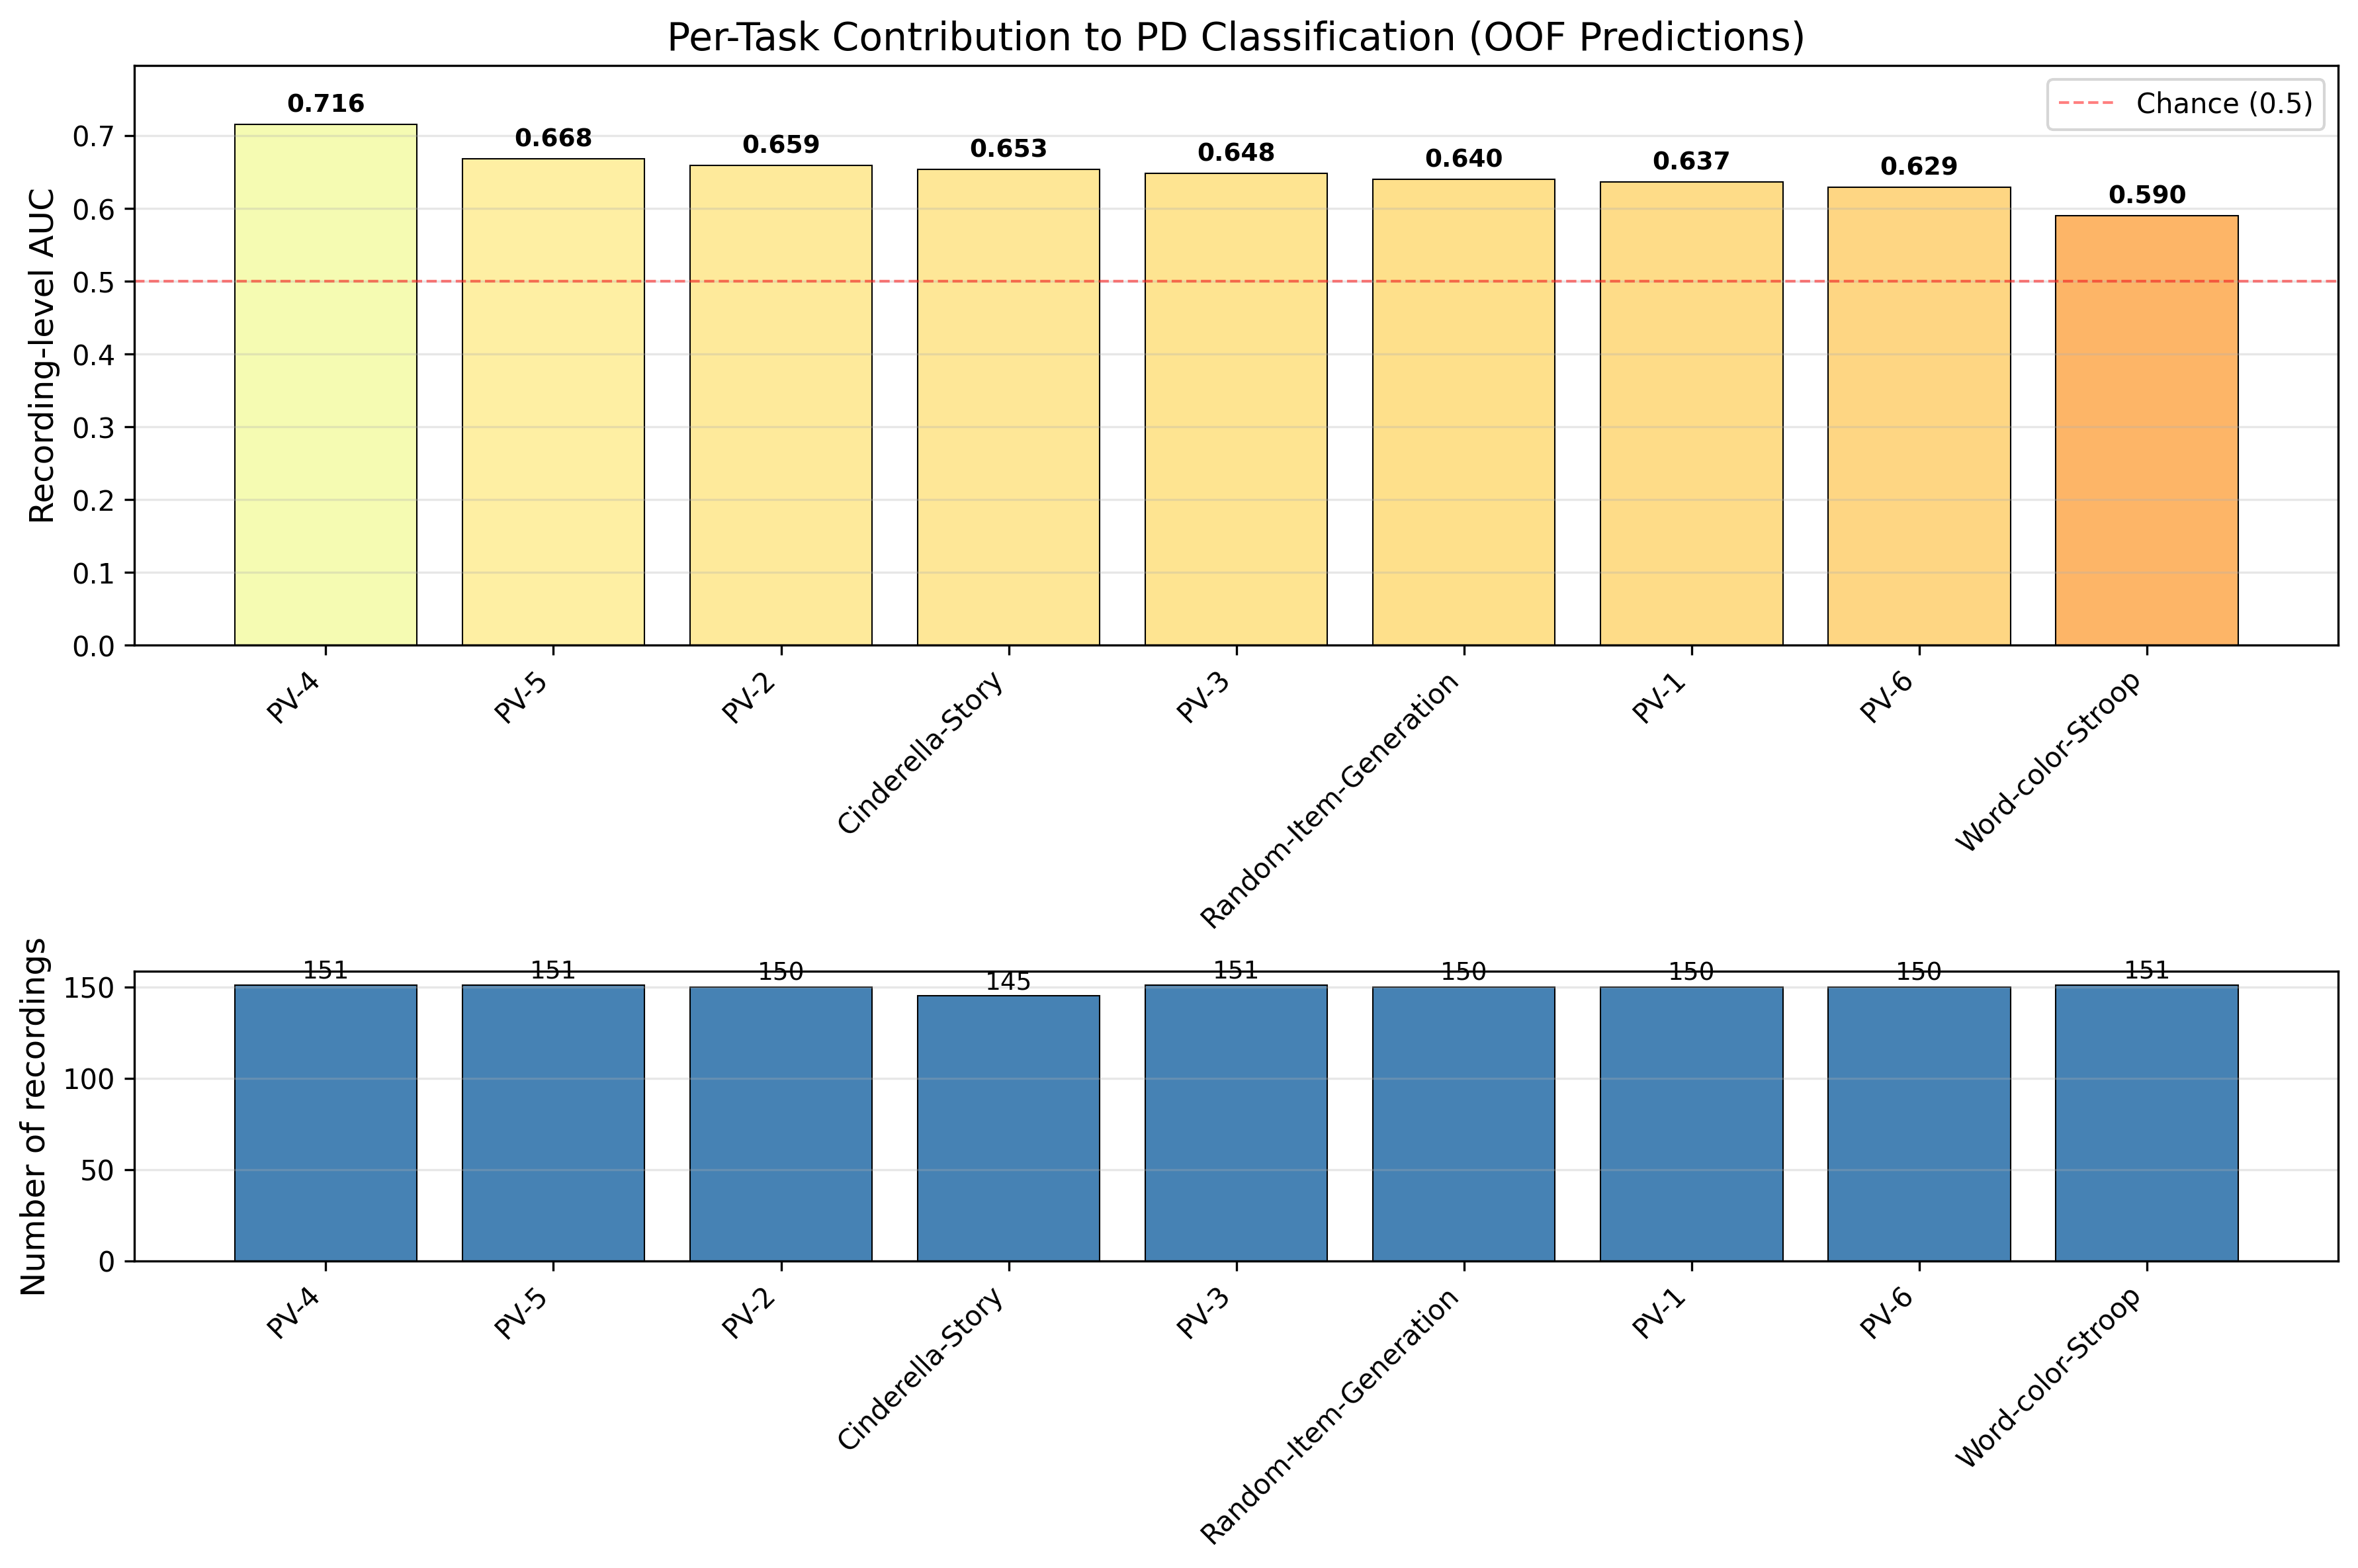
\includegraphics[width=0.85\textwidth]{per_task_contribution.png}
\caption{\textbf{Supplementary Figure S3. Per-task contribution to PD classification.}
Recording-level out-of-fold AUC for each of the nine selected speech tasks (top panel) and the number of recordings per task (bottom panel). All tasks exceeded chance-level discrimination (AUC $>$ 0.5, dashed red line). Productive Vocabulary 4 (PV-4) achieved the highest recording-level AUC (0.716), suggesting that lexical retrieval under time pressure elicits motor speech patterns most discriminative for PD. Word-Color Stroop achieved the lowest AUC (0.590), indicating that executive function demands are less informative for PD detection from spectrograms alone. The relatively uniform sample sizes across tasks ($\sim$145--151 recordings) support fair comparison.}
\label{fig:pertask}
\end{figure}


%% ============================================================
%% SECTION 3: SUPPLEMENTARY TABLES
%% ============================================================
\newpage
\section{Supplementary Tables}

%% --- TABLE S1: BASELINE COMPARISON ---
\begin{table}[H]
\centering
\caption{\textbf{Supplementary Table S1. Baseline and ablation comparison for PD screening (selected tasks, participant-level, out-of-fold).} All models used identical five-fold cross-validation splits (random\_state = 42, n = 112 participants). The fine-tuned AST with SpecAugment achieved the highest OOF AUC (0.772), outperforming all baselines and the no-augmentation ablation.}
\label{tab:baseline}
\vspace{0.5em}
\begin{tabular}{L{4.5cm} C{2cm} C{1.5cm} C{1.5cm} C{1.5cm} C{1.5cm} C{1.5cm}}
\toprule
\textbf{Model} & \textbf{Trainable Params} & \textbf{OOF AUC} & \textbf{OOF F1} & \textbf{OOF Recall} & \textbf{OOF Prec.} & \textbf{Time} \\
\midrule
Fine-tuned AST + SpecAug & 86.4M (100\%) & \textbf{0.772} & 0.769 & 0.847 & 0.704 & 68 min \\
ResNet18 (ImageNet) & 11.3M (100\%) & 0.722 & 0.660 & 0.542 & 0.842 & 7 min \\
Fine-tuned AST (no SpecAug) & 86.4M (100\%) & 0.714 & 0.732 & 0.763 & 0.703 & 161 min \\
Frozen AST (linear probe) & 199K (0.23\%) & 0.681 & 0.712 & 0.712 & 0.712 & 68 min \\
Logistic Regression & 810 & 0.598 & 0.613 & 0.576 & 0.654 & $<$1 min \\
\bottomrule
\end{tabular}
\end{table}

\vspace{2em}

%% --- TABLE S2: CROSS-STUDY COMPARISON ---
\begin{table}[H]
\centering
\caption{\textbf{Supplementary Table S2. Cross-study comparison of voice-based screening approaches.} Direct numerical comparison is limited by differences in datasets, cohort sizes, evaluation protocols, and metrics. Studies using recording-level evaluation are expected to report higher performance due to within-subject correlation.}
\label{tab:crossstudy}
\vspace{0.5em}
\small
\begin{tabular}{L{2.2cm} L{1.8cm} L{2cm} L{2.2cm} C{0.8cm} L{1.8cm} L{1.8cm}}
\toprule
\textbf{Study} & \textbf{Condition} & \textbf{Model} & \textbf{Dataset} & \textbf{N} & \textbf{Eval Level} & \textbf{Metric} \\
\midrule
This work & PD & AST (fine-tuned) & Bridge2AI v2.0 & 112 & Participant, OOF & AUC 0.772 \\
This work & PD & ResNet18 (CNN) & Bridge2AI v2.0 & 112 & Participant, OOF & AUC 0.722 \\
This work & PD & AST (frozen) & Bridge2AI v2.0 & 112 & Participant, OOF & AUC 0.681 \\
This work & PD & Log.\ Regression & Bridge2AI v2.0 & 112 & Participant, OOF & AUC 0.598 \\
Amato 2024 & PD & AST & PC-GITA / ITA & 150 & Recording & 92--97\% acc \\
MARVEL 2025 & Neurological & Multi-task & Bridge2AI v2.0 & 442 & Participant & AUROC 0.89 \\
\midrule
This work & Dementia & AST (fine-tuned) & Bridge2AI v2.0 & 112 & Participant, OOF & AUC 0.779 \\
ADReSS 2020 & Dementia & Various & DementiaBank & $\sim$156 & Participant & $\sim$79\% acc \\
\midrule
This work & Depression & AST (fine-tuned) & Bridge2AI v2.0 & 90 & Participant, OOF & AUC 0.632 \\
AMAST 2025 & Depression & Modified AST & DAIC-WOZ & $\sim$189 & Participant & F1 $>$ 0.90 \\
\bottomrule
\end{tabular}
\end{table}

\vspace{2em}

%% --- TABLE S3: COMORBIDITY ---
\begin{table}[H]
\centering
\caption{\textbf{Supplementary Table S3. Comorbidity cross-tabulation across all 442 Bridge2AI v2.0.0 participants.} Labels derived from self-reported phenotype data. Low overlap across conditions supports the interpretation that models learn condition-specific acoustic patterns rather than shared symptom profiles.}
\label{tab:comorbidity}
\vspace{0.5em}

\textbf{(a) Parkinson's Disease $\times$ Dementia}
\vspace{0.3em}

\begin{tabular}{l C{2cm} C{2cm} C{1.5cm}}
\toprule
 & \textbf{Dementia+} & \textbf{Dementia$-$} & \textbf{Total} \\
\midrule
PD+ & 2 & 59 & 61 \\
PD$-$ & 40 & 341 & 381 \\
\midrule
Total & 42 & 400 & 442 \\
\bottomrule
\end{tabular}

\vspace{1.5em}

\textbf{(b) Parkinson's Disease $\times$ Depression}
\vspace{0.3em}

\begin{tabular}{l C{2.2cm} C{2.2cm} C{1.5cm}}
\toprule
 & \textbf{Depression+} & \textbf{Depression$-$} & \textbf{Total} \\
\midrule
PD+ & 3 & 58 & 61 \\
PD$-$ & 49 & 332 & 381 \\
\midrule
Total & 52 & 390 & 442 \\
\bottomrule
\end{tabular}

\vspace{1.5em}

\textbf{(c) Dementia $\times$ Depression}
\vspace{0.3em}

\begin{tabular}{l C{2.2cm} C{2.2cm} C{1.5cm}}
\toprule
 & \textbf{Depression+} & \textbf{Depression$-$} & \textbf{Total} \\
\midrule
Dementia+ & 5 & 37 & 42 \\
Dementia$-$ & 47 & 353 & 400 \\
\midrule
Total & 52 & 390 & 442 \\
\bottomrule
\end{tabular}
\end{table}

\vspace{2em}

%% --- TABLE S4: CALIBRATION ---
\begin{table}[H]
\centering
\caption{\textbf{Supplementary Table S4. Calibration assessment (Brier scores) from out-of-fold predictions.} Lower scores indicate better calibration (range 0--1). The dementia model showed the best calibration; the depression model showed the poorest, consistent with the instability of its predictions.}
\label{tab:brier}
\vspace{0.5em}
\begin{tabular}{l C{2cm} C{2cm} C{2cm}}
\toprule
 & \textbf{PD} & \textbf{Dementia} & \textbf{Depression} \\
\midrule
OOF AUC-ROC & 0.772 & 0.779 & 0.632 \\
Brier Score & 0.204 & 0.188 & 0.248 \\
\bottomrule
\end{tabular}
\end{table}

\vspace{2em}

%% --- TABLE S5: PER-TASK ---
\begin{table}[H]
\centering
\caption{\textbf{Supplementary Table S5. Per-task recording-level AUC for PD classification (selected tasks).} Recording-level out-of-fold AUC computed separately for each task. All tasks exceeded chance (0.5). Productive Vocabulary 4 was the most discriminative individual task.}
\label{tab:pertask}
\vspace{0.5em}
\begin{tabular}{l C{2cm} C{1.5cm} C{1.5cm} C{2.5cm}}
\toprule
\textbf{Task} & \textbf{Recordings} & \textbf{PD+} & \textbf{PD$-$} & \textbf{Recording AUC} \\
\midrule
Productive Vocabulary 4 & 151 & 85 & 66 & 0.716 \\
Productive Vocabulary 5 & 151 & 85 & 66 & 0.668 \\
Productive Vocabulary 2 & 150 & 84 & 66 & 0.659 \\
Cinderella Story & 145 & 81 & 64 & 0.653 \\
Productive Vocabulary 3 & 151 & 85 & 66 & 0.648 \\
Random Item Generation & 150 & 84 & 66 & 0.640 \\
Productive Vocabulary 1 & 150 & 85 & 65 & 0.637 \\
Productive Vocabulary 6 & 150 & 84 & 66 & 0.629 \\
Word-Color Stroop & 151 & 84 & 67 & 0.590 \\
\bottomrule
\end{tabular}
\end{table}


\end{document}
